\documentclass[]{final_report}
\usepackage{graphicx}
\usepackage{hyperref}

% Added packages
\usepackage{amsmath,amssymb}
\usepackage{booktabs}
\usepackage{xcolor}
\usepackage{tcolorbox}
\usepackage{tikz}
\usepackage{pgfplots}
\pgfplotsset{compat=1.18}

%%%%%%%%%%%%%%%%%%%%%%
%%% Input project details
\def\studentname{Botir Khaltaev}
\def\reportyear{2025}
\def\projecttitle{TensorStore: An io\_uring-Native Evolution of the ServerlessLLM Storage Engine}
\def\supervisorname{Supervisor Name}
\def\degree{BSc (Hons) in Computer Science}
\def\fullOrHalfUnit{Full Unit}
\def\finalOrInterim{Interim Report}

\pgfplotsset{
    every axis/.append style={
        yticklabel style={/pgf/number format/fixed},
        scaled y ticks=false
    }
}


\begin{document}

\maketitle

%%%%%%%%%%%%%%%%%%%%%%
%%% Declaration

\chapter*{Declaration}

This report has been prepared on the basis of my own work. Where other published and unpublished source materials have been used, these have been acknowledged.

\vskip3em

Word Count: 4537

\vskip3em

Student Name: \studentname

\vskip3em

Date of Submission: 19/12/2025

\vskip3em

Signature: BK

\newpage

%%%%%%%%%%%%%%%%%%%%%%
%%% Table of Contents
\tableofcontents
\pdfbookmark[0]{Table of Contents}{toc}
\newpage

%%%%%%%%%%%%%%%%%%%%%%
%%% Abstract

\begin{abstract}

Serverless and multi-tenant inference systems increasingly rely on loading large model checkpoints on demand. In these environments, cold-start latency is often dominated by checkpoint loading rather than by model execution. Although modern NVMe storage provides high peak throughput, practical loading performance frequently falls short of hardware limits.

This project investigates checkpoint loading as an I/O submission problem. A prototype loader, TensorStore, is implemented with multiple I/O backends; this interim report evaluates synchronous POSIX I/O and Linux \texttt{io\_uring}, which represent two fundamentally different I/O submission models.

Using real-world Large Language Model checkpoints and fixed read request patterns, the evaluation measures effective throughput, read IOPS, and latency characteristics. Results show that synchronous I/O underutilises NVMe hardware due to blocking submission and shallow queue depth. In contrast, \texttt{io\_uring} achieves higher throughput and higher read IOPS by sustaining deeper queues and reducing submission overhead, with the largest gains observed for fragmented checkpoint layouts.

These findings indicate that checkpoint loading performance is often limited by submission strategy rather than storage bandwidth, motivating further exploration of asynchronous, kernel-backed I/O for cold-start-sensitive inference systems.

\end{abstract}




\newpage
%%%%%%%%%%%%%%%%%%%%%%
%%% Project Specification

\chapter*{Project Specification}
\addcontentsline{toc}{chapter}{Project Specification}

The purpose of this project is to examine how different I/O strategies influence the performance of Large Language Model (LLM) checkpoint loading on modern NVMe hardware. The work centres on a practical question: given realistic checkpoint formats and deployment constraints, how much improvement can be achieved by adopting Linux \texttt{io\_uring} instead of traditional I/O paths.

To answer this, a checkpoint loading framework has been developed with two I/O backends for this interim report: synchronous POSIX I/O and Linux \texttt{io\_uring}. The system operates on two checkpoint layouts, SafeTensors and a ServerlessLLM-style partitioned layout, described in Chapter~\ref{chap:background}. This enables a controlled comparison under consistent and representative workloads.


The core objectives of the project are:

\begin{itemize}
\item to build a unified, backend-agnostic loading interface capable of supporting realistic LLM checkpoint formats;
\item to implement and integrate multiple I/O strategies over the course of the project, and to evaluate synchronous POSIX I/O and Linux \texttt{io\_uring} in this interim report;
\item to develop a benchmarking harness that measures throughput, latency distributions, IOPS and device utilisation;
\item to analyse the behaviour of each backend and identify where performance is lost or gained;
\item to draw out design principles for future checkpoint formats and loader implementations aimed at predictable, high throughput loading.
\end{itemize}


\subsection*{Planning and Time-scale}
\addcontentsline{toc}{section}{Planning and Time-scale}

Work completed for this interim report focused on establishing a reproducible benchmark harness and producing a fair baseline comparison between synchronous POSIX I/O and Linux \texttt{io\_uring} using realistic checkpoint workloads.

The remaining work is organised into three sequential phases. Phase 2 is prioritised immediately after interim submission because it directly affects the validity and ceiling performance of the \texttt{io\_uring} backend used throughout the final evaluation.

\begin{itemize}
    \item \textbf{Phase 2: Runtime and crate-level improvements (Rust \texttt{io\_uring} stack).}
    Identify bottlenecks in the current Rust \texttt{io\_uring} stack used for high-throughput reads, with particular attention to \texttt{tokio-uring}. Implement changes needed by checkpoint loading workloads, including fixed buffer registration and reuse, reducing allocation and copying overhead, and improving submission efficiency at high queue depth.

    \item \textbf{Phase 3: Python integration via bindings.}
    Expose the loader interface through Python bindings so it can be used directly in typical inference stacks. This phase focuses on a stable API boundary, clear buffer ownership rules, and preserving identical byte-range request traces so that backend comparisons remain valid.

    \item \textbf{Phase 4: GPU Direct Storage style path (GDS).}
    Investigate staging checkpoint data into GPU-addressable memory where supported. This includes evaluating alignment and registration constraints and measuring whether reducing CPU-side involvement improves end-to-end cold-start latency in a realistic pipeline.
\end{itemize}

Each phase will be validated using the same benchmarking methodology as the interim evaluation, with changes assessed using effective throughput, read IOPS, and their impact on checkpoint load time.


The resulting framework and preliminary findings form the basis for the broader evaluation and analysis that will follow in the final report.
\newpage

%%%%%%%%%%%%%%%%%%%%%%
%%% Introduction


\chapter{Introduction}
\label{chap:introduction}

Large Language Models are increasingly deployed in serverless and multi-tenant environments where compute and memory resources are shared across users. Models are frequently evicted from memory to reduce cost and improve utilisation, and requests for evicted models trigger a checkpoint reload from persistent storage. For large models, checkpoint loading can dominate user-visible cold-start latency.

This project evaluates checkpoint loading as an I/O submission problem. It compares synchronous POSIX I/O with Linux \texttt{io\_uring} using TensorStore, a prototype loader that replays identical byte-range read requests derived from checkpoint metadata across both backends. This isolates the effect of submission behaviour on effective throughput, read IOPS, and latency under sequential and fragmented checkpoint layouts.

The remainder of this report is structured as follows. Chapter~\ref{chap:background} introduces checkpoint loading and Linux I/O models. Chapter~\ref{chap:design} describes TensorStore. Chapter~\ref{chap:evaluation} presents preliminary results. Chapter~\ref{chap:discussion} discusses implications and future work.



\newpage

%%%%%%%%%%%%%%%%%%%%%%
%%% Background and Motivation

\chapter{Background and Motivation}
\label{chap:background}

Checkpoint loading is a critical component of cold-start behaviour in serverless and multi-tenant inference systems. When a model is evicted from memory, inference cannot begin until the required parameters are staged from persistent storage into main memory. For large models, this loading step can dominate startup latency.

Checkpoint loading is constrained by access patterns defined by checkpoint metadata. Tensor offsets and sizes impose fixed read ranges that must be respected, which limits the ability of loaders to arbitrarily merge or reorder requests. As a result, loading performance depends not only on storage bandwidth but also on how effectively read requests are submitted and overlapped.

\section{Checkpoint Loading as an I/O Problem}

Checkpoint loading is fundamentally an I/O-intensive workload. A loader issues a fixed set of read operations derived from checkpoint metadata, often across multiple files and non-contiguous byte ranges. Unlike streaming workloads, these reads cannot be freely coalesced because tensor boundaries and offsets must be preserved.

In this setting, effective throughput depends on the ability to sustain sufficient concurrency. If read requests are issued serially or with limited overlap, the storage device cannot fully exploit its internal parallelism. This leads to underutilisation even when the underlying medium is capable of much higher performance~\cite{NVME_SPEC,STORAGE_QUEUEING}.

\section{Limitations of Traditional Synchronous I/O}

The POSIX I/O model is based on blocking system calls such as \texttt{read()}. Each call enters the kernel and blocks the issuing thread until completion. While this model is simple and widely used, it tightly couples submission and completion.

For workloads consisting of many read operations, this coupling limits achievable concurrency. Even when multiple threads are used, each operation incurs syscall overhead and issuing threads spend time blocked waiting for completion. As a result, the effective queue depth observed by the storage device is often shallow, leading to idle periods and reduced throughput~\cite{LINUX_KERNEL_DEVELOPMENT,LINUX_BLOCK_LAYER}.

These effects become more pronounced for fragmented checkpoint layouts. Partitioned formats increase the number of read operations and file descriptor switches, amplifying submission overhead and increasing sensitivity to scheduling delays.

\section{Asynchronous I/O and \texttt{io\_uring}}

Linux \texttt{io\_uring} provides an asynchronous I/O interface designed to reduce per-operation overhead and support deeper queueing. Applications prepare I/O requests in shared memory rings and submit them to the kernel in batches, while completion events are delivered separately~\cite{AXBOE_IOURING_PDF,MAN7_IOURING7}.

This decoupling allows applications to maintain many outstanding read requests without blocking issuing threads. From the perspective of the storage device, this enables deeper queues and more continuous utilisation. Modern NVMe devices are designed to exploit internal parallelism through multiple submission and completion queues, which requires sustained outstanding I/O to achieve high effective throughput~\cite{NVME_SPEC,STORAGE_QUEUEING}.

Based on this model, an asynchronous submission mechanism that sustains higher queue depth is expected to achieve higher throughput and higher read IOPS for checkpoint loading workloads, particularly when access patterns are fragmented.

\section{Motivation for This Project}

Despite the availability of asynchronous I/O interfaces, many checkpoint loaders continue to rely on synchronous or thread-based I/O models. In practice, it is not always clear whether the additional complexity of asynchronous submission yields consistent benefits for real checkpoint workloads defined by fixed metadata layouts.

The motivation for this project is to evaluate whether Linux \texttt{io\_uring} can outperform synchronous POSIX I/O when loading modern LLM checkpoints under realistic access patterns. By replaying identical byte-range read requests across backends, the evaluation isolates the effect of I/O submission strategy from storage hardware and checkpoint format.

Understanding these trade-offs is important for the design of inference systems operating under strict cold-start latency constraints.



%%%%%%%%%%%%%%%%%%%%%%
%%% Related Work

\chapter{Related Work}
\label{chap:related}

This project lies at the intersection of model checkpoint management and operating system I/O mechanisms. Prior work in this area can be grouped into checkpoint format design, serverless inference system architecture, and operating system support for high-performance I/O. This chapter reviews these strands and positions the present work relative to them.

\section{Checkpoint Formats and Model Storage}

Several checkpoint formats aim to improve model portability, safety, and loading behaviour. SafeTensors introduces a memory-safe format that stores tensor metadata alongside contiguous tensor data, enabling predictable access patterns and avoiding unsafe deserialisation~\cite{safetensors_docs}. Other approaches partition checkpoints across multiple files to support modular loading, distribution, or fault isolation, as seen in systems such as ServerlessLLM~\cite{FU:2024,serverlessllm_repo}.

While checkpoint formats influence access patterns, they do not guarantee efficient loading. Even largely sequential layouts can perform poorly if read requests are issued with insufficient concurrency. This project therefore treats checkpoint layout as an input constraint and focuses on how read requests are submitted to the operating system.

\section{Serverless and Multi-Tenant Inference Systems}

Recent work on serverless and multi-tenant inference systems identifies checkpoint loading as a major contributor to cold-start latency. Systems such as ServerlessLLM evaluate architectural techniques including model partitioning, caching, and placement strategies to reduce startup time and improve resource utilisation~\cite{FU:2024}.

These studies typically evaluate end-to-end latency and throughput, treating storage access as one component of a larger pipeline. While they demonstrate the importance of checkpoint loading, they do not examine low-level I/O submission mechanisms in isolation. The present project complements this work by analysing checkpoint loading as a systems problem and evaluating how operating system I/O models affect storage utilisation under realistic workloads.

\section{Asynchronous I/O in Linux}

Asynchronous I/O has long been available in Linux through interfaces such as POSIX AIO and native Linux AIO. In practice, these interfaces have seen limited adoption for high-throughput workloads due to overhead, complex semantics, and limited scalability when issuing large numbers of requests~\cite{MAN7_AIO7,MAN7_IO_SETUP2,MAN7_IO_SUBMIT2}.

Linux \texttt{io\_uring} was introduced to address these limitations by providing a shared-memory interface for I/O submission and completion, reducing syscall overhead and enabling efficient batching~\cite{AXBOE_IOURING_PDF,MAN7_IOURING7}. Prior work shows that \texttt{io\_uring} can outperform traditional I/O interfaces for workloads that benefit from deep queueing and high request concurrency, including databases and storage-intensive applications.

This project extends this line of work by applying \texttt{io\_uring} to LLM checkpoint loading. Rather than relying on synthetic microbenchmarks, it evaluates real checkpoint layouts and fixed read request patterns.

\section{Positioning of This Work}

Unlike work that focuses on new checkpoint formats or complete inference pipelines, this project isolates checkpoint loading as an I/O submission problem. By replaying identical byte-range workloads across synchronous POSIX I/O and \texttt{io\_uring}, it provides a controlled comparison of how submission strategy affects storage utilisation.

This focus allows observed performance differences to be attributed directly to the I/O model rather than to checkpoint parsing, memory allocation, or scheduling policies.




%%%%%%%%%%%%%%%%%%%%%%
%%% Design and Implementation

\chapter{Design and Implementation}
\label{chap:design}

TensorStore was designed to enable a controlled and reproducible comparison of I/O submission strategies for checkpoint loading. The primary requirement is that, given identical checkpoint metadata, each backend executes the same set of byte-range read requests and is evaluated using the same measurement path. The design therefore emphasises separation between checkpoint parsing, I/O submission, and benchmarking.

\section{System Architecture}

\begin{figure}[h]
\centering
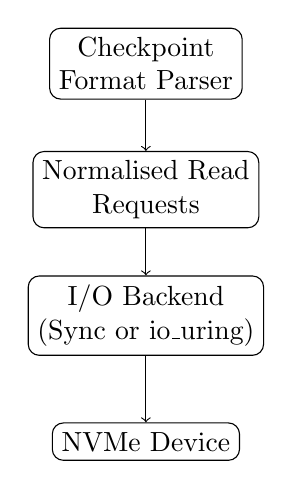
\begin{tikzpicture}[
    node distance=1.6cm,
    every node/.style={draw, rounded corners, align=center}
]
\node (format) {Checkpoint\\Format Parser};
\node (iface) [below of=format] {Normalised Read\\Requests};
\node (backend) [below of=iface] {I/O Backend\\(Sync or io\_uring)};
\node (device) [below of=backend] {NVMe Device};

\draw[->] (format) -- (iface);
\draw[->] (iface) -- (backend);
\draw[->] (backend) -- (device);
\end{tikzpicture}
\caption{TensorStore architecture showing separation between format parsing, backend execution, and storage access.}
\label{fig:tensorstore-arch}
\end{figure}

TensorStore is structured into three layers:

\begin{itemize}
    \item a format layer that parses checkpoint metadata and produces a normalised set of read requests;
    \item a backend layer that issues read operations using a specific I/O submission model;
    \item an evaluation harness that executes workloads and records performance metrics.
\end{itemize}

This structure ensures that observed performance differences can be attributed to the I/O model rather than to parsing logic or measurement artefacts.

\section{Backend Interface}

All backends implement a shared interface based on explicit ranged reads. Each request specifies a file path, a byte offset, and a length. Backends must execute requests exactly as specified and are not permitted to merge, split, or reorder ranges.

This constraint ensures a fair comparison. Performance differences therefore reflect submission behaviour rather than changes to the workload.

\section{Synchronous POSIX Backend}

The synchronous backend issues blocking \texttt{read()} calls through the POSIX I/O interface. For large files, reads are split into fixed-size chunks to enable limited parallelism using multiple threads.

Each read incurs a syscall and blocks the issuing thread until completion. Even when multiple threads are used, submission and completion remain tightly coupled, which limits the number of outstanding requests that can be maintained concurrently. Under fragmented workloads, this results in shallow effective queue depth and increased sensitivity to scheduling overhead.

This backend serves as a realistic baseline against which asynchronous submission mechanisms can be evaluated.

\section{Buffer Pool and Memory Management}

TensorStore uses a reusable buffer pool to avoid per-read allocation overhead and to support aligned buffers where possible. Buffers are allocated during initialisation and recycled across read operations.

When alignment constraints are satisfied, buffers are used directly for I/O. When alignment cannot be guaranteed, the loader falls back to buffered I/O while preserving the same logical read requests. This ensures that unaligned tensor ranges do not invalidate backend comparisons.

\section{Checkpoint Format Support}

The format layer parses checkpoint metadata and produces a normalised representation consisting of file paths and byte ranges. This isolates format-specific parsing logic from the I/O path and allows the same workload to be replayed across different backends.

\subsection{SafeTensors}

\begin{figure}[h]
    \centering
    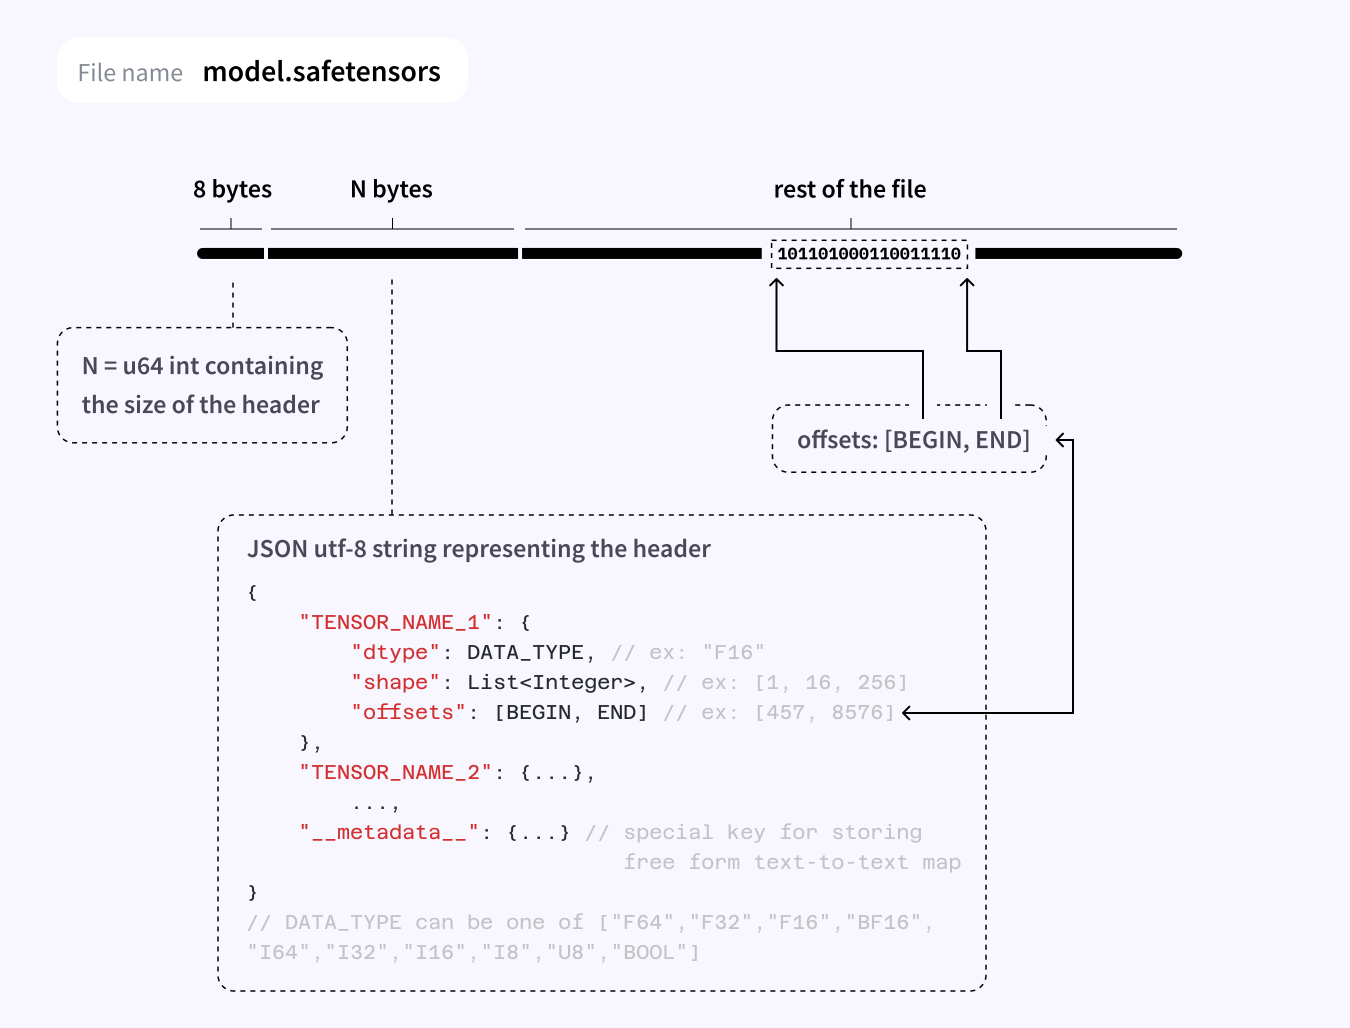
\includegraphics[width=0.75\textwidth]{safetensors-layout.png}
    \caption{Simplified SafeTensors layout, adapted from the Hugging Face SafeTensors documentation~\cite{safetensors_docs}.}
    \label{fig:safetensors-layout}
\end{figure}

SafeTensors stores tensor data in a single file with a metadata header. Once the header is parsed, tensor offsets can be computed directly. This produces a largely sequential access pattern, which is useful for evaluating backend behaviour when fragmentation is minimal.

\subsection{ServerlessLLM-Style Partitioned Format}

\begin{figure}[h]
    \centering
    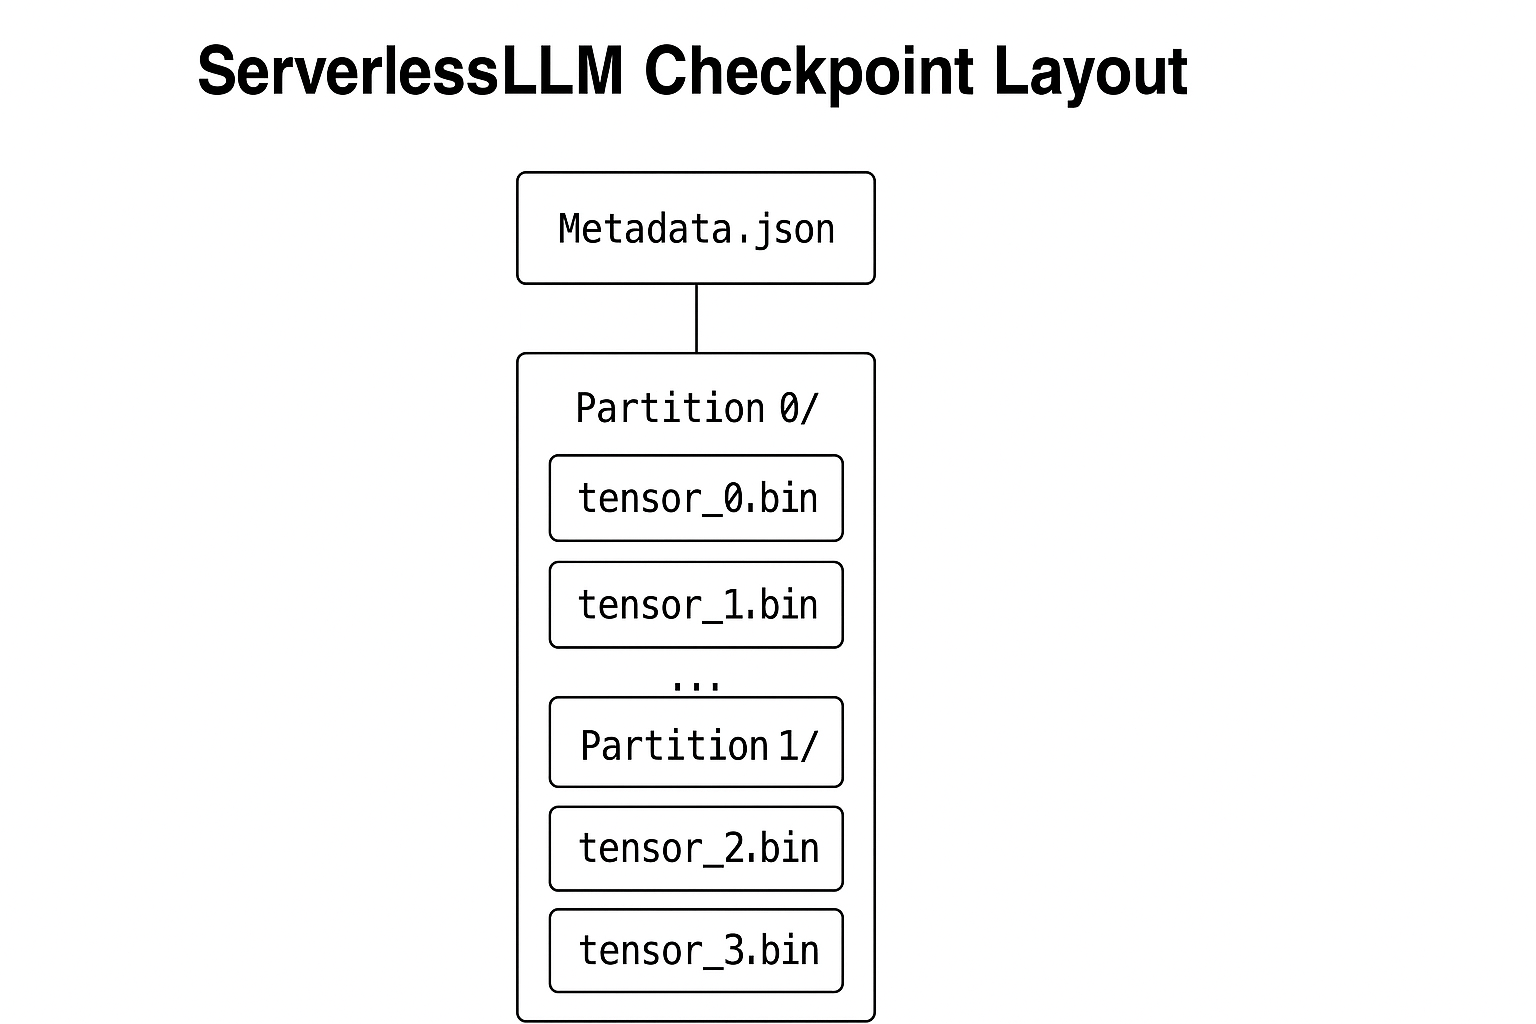
\includegraphics[width=0.75\textwidth]{serverlessllm-layout.png}
    \caption{Overview of the ServerlessLLM partitioned checkpoint structure~\cite{FU:2024}.}
    \label{fig:serverlessllm-layout}
\end{figure}

In the partitioned format, tensor ranges are distributed across multiple files. This increases the number of read operations and file descriptor switches, placing greater stress on the submission path and queue management.

\section{Evaluation Harness}

The evaluation harness executes the normalised read requests against each backend and records wall-clock load time, effective throughput, read IOPS, and basic per-read latency statistics. A warm-up phase precedes measurement runs, and repeated runs are used to ensure stable results.

Benchmarking code is kept separate from loader logic to prevent measurement artefacts and to ensure identical workloads across backends.

\section{Summary}

The design of TensorStore ensures that each I/O backend is evaluated against the same logical workload and measurement path. By isolating checkpoint parsing, I/O submission, and benchmarking, the framework provides a sound basis for analysing how different I/O models affect checkpoint loading performance.



\newpage

%%%%%%%%%%%%%%%%%%%%%%
%%% Preliminary Evaluation

\chapter{Preliminary Evaluation}
\label{chap:evaluation}

This chapter presents an empirical evaluation of TensorStore under realistic checkpoint loading workloads. The evaluation focuses on metrics that directly influence cold-start latency in serverless and multi-tenant inference systems, namely effective throughput, read IOPS, and latency behaviour.

Although TensorStore is designed to support multiple backends, this interim evaluation compares only synchronous POSIX I/O and Linux \texttt{io\_uring}. These backends represent two fundamentally different I/O submission models. Restricting the scope allows the impact of submission strategy to be isolated without introducing additional variables.

All measurements reported in this chapter are obtained by replaying identical byte-range read requests derived from checkpoint metadata. Performance differences therefore reflect the behaviour of the I/O mechanism rather than differences in access pattern or request structure.

\section{Experimental Setup}

All experiments were conducted on a single Linux system to minimise variability. The system was equipped with an Intel Core i9-10900K processor with 10 physical cores and 20 hardware threads, and 30~GB of RAM. Swap was enabled but did not contribute to memory pressure during benchmark runs.

Storage was provided by a Samsung 970 EVO NVMe SSD with a capacity of 500~GB. Both the system root filesystem and all benchmark checkpoints resided on this device and were formatted using ext4 with default mount options. Using a single storage device avoids variability introduced by heterogeneous storage configurations.

The system ran Ubuntu Linux with kernel version 6.17.0-8-generic. All experiments were executed on a single NUMA node. Device behaviour was monitored using \texttt{iostat} during benchmark runs to confirm sustained I/O activity and to verify that no swapping occurred.

Two real-world model checkpoints were evaluated:

\begin{itemize}
    \item \textbf{Mistral-7B}, approximately 9.9~GB on disk;
    \item \textbf{Qwen3-14B}, approximately 4.0~GB on disk.
\end{itemize}

Each checkpoint was evaluated using two layouts:

\begin{itemize}
    \item \textbf{SafeTensors}, a single-file layout producing largely sequential access;
    \item \textbf{ServerlessLLM-style partitioned layout}, consisting of multiple files and producing a fragmented access pattern.
\end{itemize}

For each configuration, TensorStore parsed checkpoint metadata to generate a fixed trace of file paths, byte offsets, and read lengths. This trace was replayed unchanged across both backends. Backends were not permitted to alter request boundaries, ordering, or grouping.

Each experiment consisted of a warm-up phase followed by repeated measurement runs. Results were recorded once throughput and read IOPS stabilised. Effective throughput is reported as total bytes loaded divided by end-to-end load time. Read IOPS are computed as the number of completed read operations divided by load time. Per-read latency measurements are used to characterise distribution shape rather than absolute device latency.

\section{Sequential Loading with SafeTensors}

The SafeTensors format produces a largely sequential access pattern once the metadata header has been parsed. This makes it a useful baseline for evaluating how effectively each backend sustains device throughput under minimal fragmentation.

\begin{figure}[h]
\centering
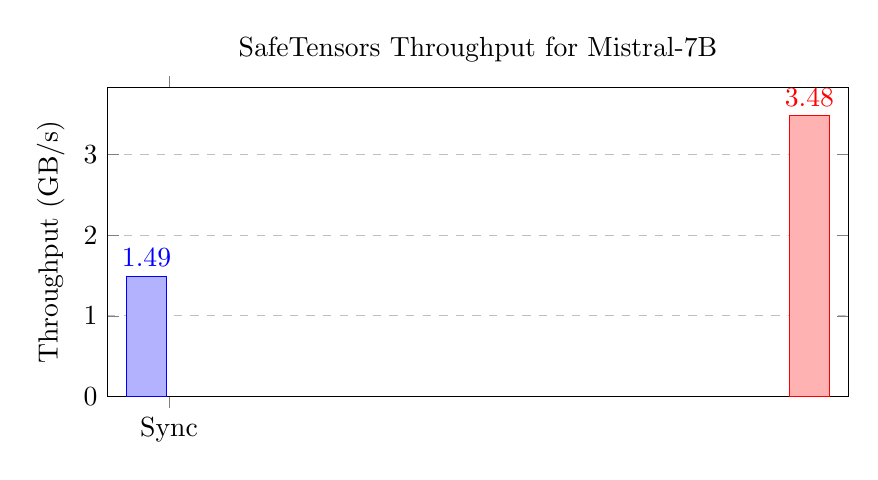
\begin{tikzpicture}
\begin{axis}[
    ybar,
    ymin=0,
    bar width=0.5cm,
    width=11cm,
    height=5.5cm,
    symbolic x coords={Sync,io\_uring},
    xtick=data,
    ylabel={Throughput (GB/s)},
    title={SafeTensors Throughput for Mistral-7B},
    nodes near coords,
    ymajorgrids=true,
    grid style=dashed,
]
\addplot coordinates {(Sync,1.49)};
\addplot coordinates {(io\_uring,3.48)};
\end{axis}
\end{tikzpicture}
\caption{Effective throughput for sequential SafeTensors loading comparing synchronous POSIX I/O and \texttt{io\_uring}.}
\label{fig:st-throughput-mistral-eval}
\end{figure}

Figure~\ref{fig:st-throughput-mistral-eval} shows that synchronous POSIX I/O achieves limited throughput despite the sequential access pattern. Blocking \texttt{read()} calls and per-operation syscall overhead prevent the loader from maintaining a steady stream of outstanding requests, resulting in underutilisation of the NVMe device.

The \texttt{io\_uring} backend achieves substantially higher throughput under the same workload. This improvement arises from non-blocking submission, which allows multiple read requests to remain in flight concurrently. As a result, device queues are populated more consistently and idle gaps are reduced.

The same qualitative behaviour was observed for the Qwen3-14B checkpoint, although absolute throughput values differed due to the smaller checkpoint size. These results show that even under favourable access patterns, checkpoint loading performance is sensitive to submission strategy.

\section{Partitioned Loading with ServerlessLLM-Style Layouts}

The ServerlessLLM-style partitioned layout distributes tensor ranges across multiple files. This increases the number of read operations and introduces frequent file descriptor switches, placing greater stress on the I/O submission path.

\begin{figure}[h]
\centering
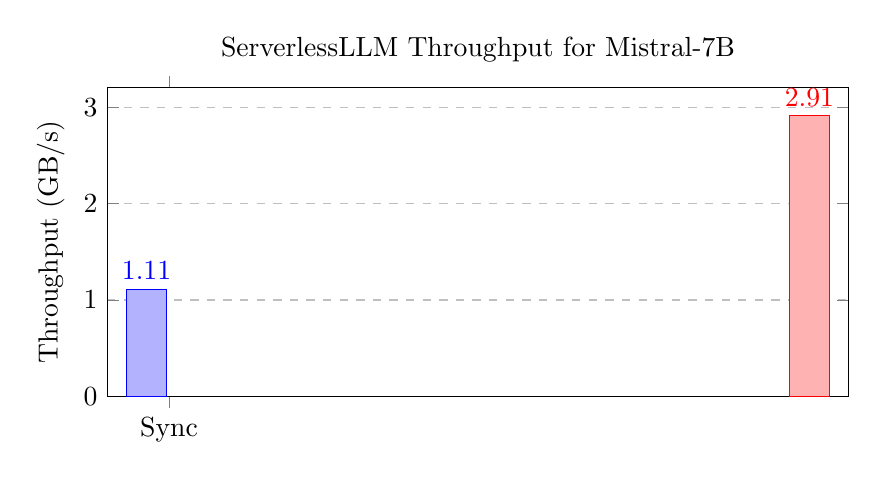
\begin{tikzpicture}
\begin{axis}[
    ybar,
    ymin=0,
    bar width=0.5cm,
    width=11cm,
    height=5.5cm,
    symbolic x coords={Sync,io\_uring},
    xtick=data,
    ylabel={Throughput (GB/s)},
    title={ServerlessLLM Throughput for Mistral-7B},
    nodes near coords,
    ymajorgrids=true,
    grid style=dashed,
]
\addplot coordinates {(Sync,1.11)};
\addplot coordinates {(io\_uring,2.91)};
\end{axis}
\end{tikzpicture}
\caption{Effective throughput for partitioned loading comparing synchronous POSIX I/O and \texttt{io\_uring}.}
\label{fig:sllm-throughput-mistral-eval}
\end{figure}

Figure~\ref{fig:sllm-throughput-mistral-eval} shows that synchronous POSIX I/O performs worse under the partitioned layout than under sequential access. Increased request count and file switching amplify submission overhead and reduce the effective queue depth that can be maintained using blocking submission.

The \texttt{io\_uring} backend sustains significantly higher throughput under the same workload. By decoupling submission from completion, it maintains a larger number of outstanding requests even as fragmentation increases. The larger performance gap relative to the SafeTensors case indicates that fragmented access patterns place greater demands on the submission mechanism.

\section{Read IOPS and Queue Utilisation}

Throughput alone does not fully describe storage device utilisation for fragmented workloads. Read IOPS provide additional insight into how effectively request queues are populated.

\begin{figure}[h]
\centering
\begin{tikzpicture}
\begin{axis}[
    ybar,
    ymin=0,
    bar width=0.45cm,
    width=11cm,
    height=5.5cm,
    symbolic x coords={Sync,io\_uring},
    xtick=data,
    ylabel={Read IOPS (ops/s)},
    title={Read IOPS for Partitioned Mistral-7B},
    nodes near coords,
    ymajorgrids=true,
    grid style=dashed,
    scaled y ticks=false,
    yticklabel style={
        /pgf/number format/fixed,
        /pgf/number format/thousands separator={,},
    }
]
\addplot coordinates {(Sync,17098)};
\addplot coordinates {(io\_uring,44669)};
\end{axis}
\end{tikzpicture}
\caption{Read IOPS for the partitioned checkpoint workload comparing synchronous POSIX I/O and \texttt{io\_uring}.}
\label{fig:sllm-iops-mistral-eval}
\end{figure}

Figure~\ref{fig:sllm-iops-mistral-eval} shows that the \texttt{io\_uring} backend sustains more than twice the read IOPS of the synchronous backend. This indicates that a larger number of requests remain outstanding, allowing the NVMe device to exploit its internal parallelism more effectively.

In contrast, synchronous POSIX I/O exhibits lower read IOPS due to blocking submission and thread scheduling delays. As request counts increase, these effects limit queue depth and cause intermittent device idle time.

\section{Latency Characteristics}

Latency was measured at the granularity of individual read operations using timestamps recorded by the evaluation harness. These measurements capture application-observed latency rather than raw device latency.

Synchronous POSIX I/O exhibits wider latency distributions with heavier tails. Because each \texttt{read()} call blocks until completion, slow reads delay subsequent submissions, producing head-of-line blocking effects.

The \texttt{io\_uring} backend produces tighter latency distributions. Submission is decoupled from completion, allowing new requests to be issued even when some reads experience higher latency. This reduces sensitivity to outlier operations and improves progress under variable I/O conditions.

\section{Summary}

This evaluation demonstrates clear differences between synchronous POSIX I/O and Linux \texttt{io\_uring} under identical checkpoint loading workloads.

Across both layouts, synchronous POSIX I/O underutilises NVMe hardware due to blocking submission and limited concurrency. These effects are present even for largely sequential access patterns and become more pronounced as fragmentation increases.

In contrast, the \texttt{io\_uring} backend sustains higher throughput and higher read IOPS by maintaining deeper queues and overlapping request execution. The performance gap is modest for SafeTensors layouts and substantially larger for ServerlessLLM-style partitioned checkpoints, supporting the conclusion that checkpoint loading performance is increasingly constrained by I/O submission strategy as fragmentation increases.


%%%%%%%%%%%%%%%%%%%%%%
%%% Discussion and Future Work

\chapter{Discussion and Future Work}
\label{chap:discussion}

This chapter interprets the preliminary evaluation results and relates them back to the theoretical expectations discussed earlier in the report. Rather than restating measured values, the focus is on explaining why the observed performance differences arise and what they imply for the design of checkpoint loaders in cold-start-sensitive inference systems.

\section{Interpretation of Results}

Across both checkpoint layouts, Linux \texttt{io\_uring} consistently achieves higher effective throughput and higher read IOPS than synchronous POSIX I/O. The central observation is that this improvement is driven by differences in request submission behaviour rather than by changes in storage hardware or access pattern.

Synchronous POSIX I/O relies on blocking \texttt{read()} calls. Each issuing thread waits for completion before submitting further requests, tightly coupling submission and completion. Even when multiple threads are used, this structure limits the number of outstanding requests and makes it difficult to maintain sustained queue depth. As a result, NVMe submission queues are populated intermittently, leading to idle periods and reduced device utilisation.

In contrast, \texttt{io\_uring} decouples submission from completion. Read requests can be prepared in advance and submitted in batches, while completions are handled independently. This allows a larger number of requests to remain in flight and enables more continuous utilisation of the storage device. The higher read IOPS observed for fragmented workloads are consistent with this model, since these workloads require sustained concurrency to exploit device-level parallelism.

\section{Effect of Checkpoint Layout}

Checkpoint layout has a direct influence on how strongly submission overhead affects loading performance.

For the SafeTensors layout, access patterns are largely sequential. In this case, achieving high throughput primarily requires keeping enough requests in flight to avoid idle gaps at the device level. The evaluation shows that synchronous I/O fails to do so, even under favourable access patterns, indicating that per-operation overhead and blocking behaviour remain significant bottlenecks.

The ServerlessLLM-style partitioned layout increases the number of read operations and distributes them across multiple files. This amplifies submission overhead and increases the queue depth required to sustain high throughput. Under these conditions, the performance gap between \texttt{io\_uring} and synchronous I/O widens. This supports the conclusion that checkpoint loading becomes increasingly submission bound as fragmentation increases.

\section{Implications for Checkpoint Loader Design}

Several design implications follow from these results.

First, high-performance checkpoint loaders must explicitly target sustained queue depth. Issuing reads serially or in small bursts prevents NVMe hardware from exploiting its internal parallelism, regardless of peak device bandwidth.

Second, per-operation overhead matters at the scale of modern model checkpoints. Large checkpoints consist of many tensor ranges, and mapping each range directly to a blocking \texttt{read()} call introduces substantial syscall and scheduling overhead. Reducing this overhead through batching and asynchronous submission has a measurable impact on end-to-end loading time.

Third, checkpoint format and loader design are closely coupled. Partitioned formats offer flexibility for distribution and modular loading, but they increase request count and file switching. These formats are therefore better matched to I/O backends that can efficiently batch and queue requests. Loader implementations that do not account for this interaction risk negating the intended benefits of format-level design choices.

\section{Limitations of the Current Evaluation}

This interim evaluation has several limitations. Measurements were conducted on a single hardware configuration, so absolute throughput values should not be generalised across devices. Only two checkpoints were evaluated, and further work is required to assess sensitivity to model size and tensor layout characteristics. In addition, checkpoint loading was evaluated in isolation. In a full inference pipeline, memory allocation, model initialisation, and runtime execution may introduce additional interactions that affect user-visible cold-start latency.

Despite these limitations, the observed trends are consistent across layouts and metrics. The higher read IOPS sustained by \texttt{io\_uring} provide direct evidence of improved queue utilisation, supporting the interpretation presented in this chapter.

\section{Future Work}

The next phase of this project will extend the evaluation in several directions.

Additional checkpoints and layouts will be evaluated to assess how performance scales with model size, tensor fragmentation, and request distribution. CPU profiling will be used to quantify submission overhead directly, including syscall cost, scheduling delays, and time spent preparing I/O requests.

Further work will also examine batching and queue-depth policies in more detail, including adaptive strategies that adjust concurrency based on observed device behaviour. Where alignment constraints can be satisfied, direct I/O will be evaluated as a means of reducing page-cache overhead and improving performance predictability.

Finally, TensorStore will be integrated into an end-to-end inference pipeline to measure user-visible cold-start latency. This will establish whether improvements at the I/O layer translate into practical benefits under realistic deployment conditions.

\section{Summary}

This chapter shows that the performance differences observed in the preliminary evaluation can be explained by differences in I/O submission strategy. By enabling batched, asynchronous submission and sustaining deeper queues, Linux \texttt{io\_uring} improves throughput and read IOPS, with the largest benefits appearing for fragmented checkpoint layouts.


\newpage

%%%%%%%%%%%%%%%%%%%%%%
%%% Conclusion

\chapter{Conclusion}
\label{chap:conclusion}

This interim report examined how Linux I/O submission mechanisms affect the cold-start cost of loading Large Language Model checkpoints from NVMe storage. The central finding is that checkpoint loading performance is constrained less by raw storage bandwidth and more by how effectively the loader submits and overlaps I/O requests.

To enable a controlled comparison, a prototype framework, TensorStore, was developed to evaluate checkpoint loading backends under identical byte-range workloads derived from checkpoint metadata. Both a sequential single-file layout (SafeTensors) and a fragmented multi-file layout (ServerlessLLM-style) were supported, allowing the effect of checkpoint layout to be isolated from the I/O mechanism itself.

Across both layouts, synchronous POSIX I/O underutilised NVMe hardware. Blocking submission and limited concurrency resulted in shallow effective queue depth, preventing the loader from sustaining device-level throughput even when access patterns were largely sequential. These limitations became more pronounced for fragmented layouts, where increased request counts amplified submission overhead and led to additional idle periods.

In contrast, Linux \texttt{io\_uring} achieved higher effective throughput and higher read IOPS by decoupling submission from completion and enabling batched, asynchronous I/O. By maintaining a larger number of outstanding requests, \texttt{io\_uring} sustained deeper queues and more continuous device utilisation. The largest performance gains were observed for fragmented checkpoint layouts, supporting the conclusion that checkpoint loading becomes increasingly submission bound as fragmentation increases.

These results demonstrate that I/O submission strategy plays a critical role in determining checkpoint loading performance on modern NVMe devices. They motivate further exploration of asynchronous, kernel-backed I/O techniques as a means of reducing cold-start latency in serverless and multi-tenant inference systems.

The next phase of this project will extend the evaluation across additional checkpoints and hardware configurations, quantify CPU-side submission overhead using profiling, and explore batching and queue-depth policies in more detail. Finally, TensorStore will be integrated into an end-to-end inference pipeline to assess whether improvements at the I/O layer translate into reduced user-visible cold-start latency in realistic deployment settings.



\newpage

%%%%%%%%%%%%%%%%%%%%%%
%%% Bibliography

\begin{thebibliography}{99}
\addcontentsline{toc}{chapter}{Bibliography}

\bibitem{COHEN:2013}
Dave Cohen and Carlos Matos.
\emph{Third Year Projects: Rules and Guidelines}.
Royal Holloway, University of London, 2013.

\bibitem{FU:2024}
Yao Fu, Leyang Xue, Yeqi Huang, Andrei-Octavian Brabete, Dmitrii Ustiugov, Yuvraj Patel, and Luo Mai.
\emph{ServerlessLLM: Low-Latency Serverless Inference for Large Language Models}.
In \emph{Proceedings of the 18th USENIX Symposium on Operating Systems Design and Implementation (OSDI 2024)}, 2024.
Available at: \url{https://www.usenix.org/system/files/osdi24-fu.pdf}

\bibitem{serverlessllm_repo}
ServerlessLLM Contributors.
\emph{ServerlessLLM}.
GitHub repository.
Available at: \url{https://github.com/ServerlessLLM/ServerlessLLM}

\bibitem{safetensors_docs}
Hugging Face.
\emph{SafeTensors Documentation}.
Available at: \url{https://huggingface.co/docs/safetensors}

\bibitem{AXBOE_IOURING_PDF}
Jens Axboe.
\emph{Efficient I/O with io\_uring}.
Online document (PDF), 2019.
Available at: \url{https://kernel.dk/io_uring.pdf}

\bibitem{MAN7_IOURING7}
Michael Kerrisk and contributors.
\emph{io\_uring(7) Linux Manual Page}.
Available at: \url{https://man7.org/linux/man-pages/man7/io_uring.7.html}

\bibitem{MAN7_IOURING_SETUP2}
Michael Kerrisk and contributors.
\emph{io\_uring\_setup(2) Linux Manual Page}.
Available at: \url{https://man7.org/linux/man-pages/man2/io_uring_setup.2.html}

\bibitem{MAN7_IOURING_ENTER2}
Michael Kerrisk and contributors.
\emph{io\_uring\_enter(2) Linux Manual Page}.
Available at: \url{https://man7.org/linux/man-pages/man2/io_uring_enter.2.html}

\bibitem{MAN7_IOURING_REGISTER2}
Michael Kerrisk and contributors.
\emph{io\_uring\_register(2) Linux Manual Page}.
Available at: \url{https://man7.org/linux/man-pages/man2/io_uring_register.2.html}

\bibitem{LIBURING_REGISTER_MAN}
Jens Axboe and contributors.
\emph{liburing: io\_uring\_register(2) man page source}.
(Repository manpage for registration and buffer-related operations.)
Available at: \url{https://github.com/axboe/liburing/blob/master/man/io_uring_register.2}

\bibitem{MAN7_OPEN2_ODIRECT}
Michael Kerrisk and contributors.
\emph{open(2) Linux Manual Page}.
(See flags including \texttt{O\_DIRECT} and related semantics.)
Available at: \url{https://man7.org/linux/man-pages/man2/open.2.html}

\bibitem{MAN7_AIO7}
Michael Kerrisk and contributors.
\emph{aio(7) Linux Manual Page}.
(Overview of POSIX AIO and Linux AIO interfaces.)
Available at: \url{https://man7.org/linux/man-pages/man7/aio.7.html}

\bibitem{MAN7_IO_SETUP2}
Michael Kerrisk and contributors.
\emph{io\_setup(2) Linux Manual Page}.
(Linux native asynchronous I/O context creation.)
Available at: \url{https://man7.org/linux/man-pages/man2/io_setup.2.html}

\bibitem{MAN7_IO_SUBMIT2}
Michael Kerrisk and contributors.
\emph{io\_submit(2) Linux Manual Page}.
(Linux native asynchronous I/O request submission.)
Available at: \url{https://man7.org/linux/man-pages/man2/io_submit.2.html}

\bibitem{MAN7_IO_GETEVENTS2}
Michael Kerrisk and contributors.
\emph{io\_getevents(2) Linux Manual Page}.
(Linux native asynchronous I/O completion retrieval.)
Available at: \url{https://man7.org/linux/man-pages/man2/io_getevents.2.html}

\bibitem{NVME_SPEC}
NVM Express Organization.
\emph{NVM Express Specifications}.
Available at: \url{https://nvmexpress.org/specifications/}

\bibitem{LINUX_KERNEL_DEVELOPMENT}
Robert Love.
\emph{Linux Kernel Development}.
3rd edition.
Addison-Wesley Professional (Pearson Education), 2010.
ISBN 978-0-672-32946-3.

\bibitem{LINUX_BLOCK_LAYER}
Daniel P. Bovet and Marco Cesati.
\emph{Understanding the Linux Kernel}.
3rd edition.
O'Reilly Media, 2005.

\bibitem{STORAGE_QUEUEING}
John L. Hennessy and David A. Patterson.
\emph{Computer Architecture: A Quantitative Approach}.
5th edition.
Morgan Kaufmann, 2012.

\bibitem{TOKIO_URING_DOCS}
tokio-rs and contributors.
\emph{tokio-uring (Rust crate documentation)}.
Available at: \url{https://docs.rs/tokio-uring/latest/tokio_uring/}

\bibitem{TOKIO_URING_CRATE}
tokio-rs and contributors.
\emph{tokio-uring (crates.io)}.
Available at: \url{https://crates.io/crates/tokio-uring}

\bibitem{NVIDIA_GDS_OVERVIEW}
NVIDIA.
\emph{GPUDirect Storage Documentation}.
Available at: \url{https://docs.nvidia.com/gpudirect-storage/index.html}

\bibitem{NVIDIA_GDS_API}
NVIDIA.
\emph{GPUDirect Storage API Reference Guide}.
Available at: \url{https://docs.nvidia.com/gpudirect-storage/api-reference-guide/index.html}

\end{thebibliography}



\end{document}
